\documentclass[tikz]{standalone}


\usepackage[cm]{sfmath}
\renewcommand{\familydefault}{\sfdefault}
\usepackage{sansmathaccent}

\usepackage{xcolor}

\usepackage{tikz}
\usetikzlibrary{backgrounds}

\definecolor{Dark2-A}{RGB}{ 27, 158, 119}
\definecolor{Dark2-B}{RGB}{217,  95,   2}

\definecolor{Set1-A}{RGB}{228,  26,  28}
\definecolor{Set1-B}{RGB}{ 55, 126, 184}

\tikzstyle{e}=[rounded corners,very thick,draw=white,double=black,arrows={-latex[black]}]
\tikzstyle{e-gray}=[e,draw=white,double=lightgray,arrows={-latex[lightgray]}]
\tikzset{every label/.style={rectangle,fill=none,draw=none, label distance=4pt}}

\tikzstyle{n}=[circle,fill=white,draw=white,line width=2pt,outer sep=0pt,inner sep=0pt, minimum size=4ex]
\tikzstyle{n square}=[n,rectangle,inner xsep=2pt,outer sep=2pt]

\tikzstyle{inline}=[anchor=base]
\tikzstyle{open}=[fill=Dark2-A!50]
\tikzstyle{closed}=[fill=Dark2-B!50]
\tikzstyle{conditioned}=[draw=black,line width=2pt]
\tikzstyle{unfair}=[text=Dark2-B]
\tikzstyle{bias}=[draw=Dark2-B]
\tikzstyle{unobserved}=[fill opacity=0.5]

\newcommand\innode[ 2 ]{ 
  \begin{tikzpicture}[baseline] 
      \node[inline,inner ysep=0pt,inner xsep=3pt,outer sep=0pt,opacity=0] (n) {#1}; 
      \useasboundingbox (n.north west) rectangle (n.south east);
      \node[n,minimum size=3ex,inner sep=1pt,inline,#2] {#1}; 
  \end{tikzpicture}
  }

\makeatletter
\DeclareRobustCommand{\rvdots}{%
  \vbox{
    \baselineskip4\p@\lineskiplimit\z@
    \kern-\p@
    \hbox{.}\hbox{.}\hbox{.}
  }}
\makeatother

\usetikzlibrary{calc}

\begin{document}

\tikzset{every node/.style={n square}}
\tikzset{every edge/.style={e}}
\tikzstyle{grayed}=[fill=gray!10]
\tikzset{x=1cm,y=1.5cm}

% FIRST DAG
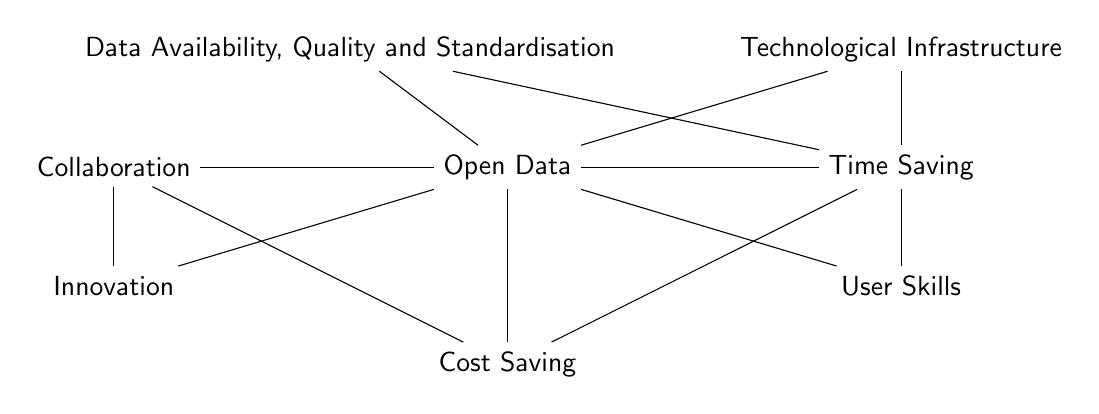
\begin{tikzpicture}

% Nodes
\node (open data)      at (-3, -1.5) {Open Data};
\node (cost saving)    at (-3,-4)    {Cost Saving};
\node (time saving)    at (2, -1.5)  {Time Saving};
\node (user skills)    at (2,-3)     {User Skills};
\node (innovation)     at (-8, -3)   {Innovation};
\node (collaboration)  at (-8, -1.5) {Collaboration};
\node (infrastructure) at (2, 0)     {Technological Infrastructure};
\node (quality)        at (-5, 0)    {Data Availability, Quality and Standardisation};

% Edges
\draw (quality)        edge (open data)
      (infrastructure) edge (open data)
      (collaboration)  edge (open data)
      (open data)      edge (cost saving)
      (open data)      edge (time saving)
      (collaboration)  edge (innovation)
      (open data)      edge (innovation)
      (collaboration)  edge (cost saving)
      (time saving)    edge (cost saving)
      (user skills)    edge (open data)
      (user skills)    edge (time saving)
      (infrastructure) edge (time saving)
      (quality)        edge (time saving);

\end{tikzpicture}

% SECOND DAG
\begin{tikzpicture}

% Nodes
\node         (open data)      at (-3, -1.5) {Open Data};
\node         (cost saving)    at (-3,-4)    {Cost Saving};
\node[closed] (time saving)    at (2, -1.5)  {Time Saving};
\node[grayed] (user skills)    at (2,-3)     {User Skills};
\node[grayed] (innovation)     at (-8, -3)   {Innovation};
\node[grayed] (collaboration)  at (-8, -1.5) {Collaboration};
\node[grayed] (infrastructure) at (2, 0)     {Technological Infrastructure};
\node[grayed] (quality)        at (-5, 0)    {Data Availability, Quality and Standardisation};

% Edges
\draw (quality)        edge[e-gray] (open data)
      (infrastructure) edge[e-gray] (open data)
      (collaboration)  edge[e-gray] (open data)
      (open data)      edge         (cost saving)
      (open data)      edge[e-gray] (time saving)
      (collaboration)  edge[e-gray] (innovation)
      (open data)      edge[e-gray] (innovation)
      (collaboration)  edge[e-gray] (cost saving)
      (time saving)    edge[e-gray] (cost saving)
      (user skills)    edge[e-gray] (open data)
      (user skills)    edge[e-gray] (time saving)
      (infrastructure) edge[e-gray] (time saving)
      (quality)        edge[e-gray] (time saving);

\end{tikzpicture}

% THIRD DAG
\begin{tikzpicture}

% Nodes
\node                   (open data)      at (-3, -1.5) {Open Data};
\node                   (cost saving)    at (-3,-4)    {Cost Saving};
\node[grayed]           (time saving)    at (2, -1.5)  {Time Saving};
\node[grayed]           (user skills)    at (2,-3)     {User Skills};
\node[open,conditioned] (innovation)     at (-8, -3)   {Innovation};
\node[open]             (collaboration)  at (-8, -1.5) {Collaboration};
\node[grayed]           (infrastructure) at (2, 0)     {Technological Infrastructure};
\node[grayed]           (quality)        at (-5, 0)    {Data Availability, Quality and Standardisation};

% Edges
\draw (quality)        edge[e-gray] (open data)
      (infrastructure) edge[e-gray] (open data)
      (collaboration)  edge         (open data)
      (open data)      edge         (cost saving)
      (open data)      edge[e-gray] (time saving)
      (collaboration)  edge         (innovation)
      (open data)      edge         (innovation)
      (collaboration)  edge         (cost saving)
      (time saving)    edge[e-gray] (cost saving)
      (user skills)    edge[e-gray] (open data)
      (user skills)    edge[e-gray] (time saving)
      (infrastructure) edge[e-gray] (time saving)
      (quality)        edge[e-gray] (time saving);

\end{tikzpicture}

% FOURTH DAG
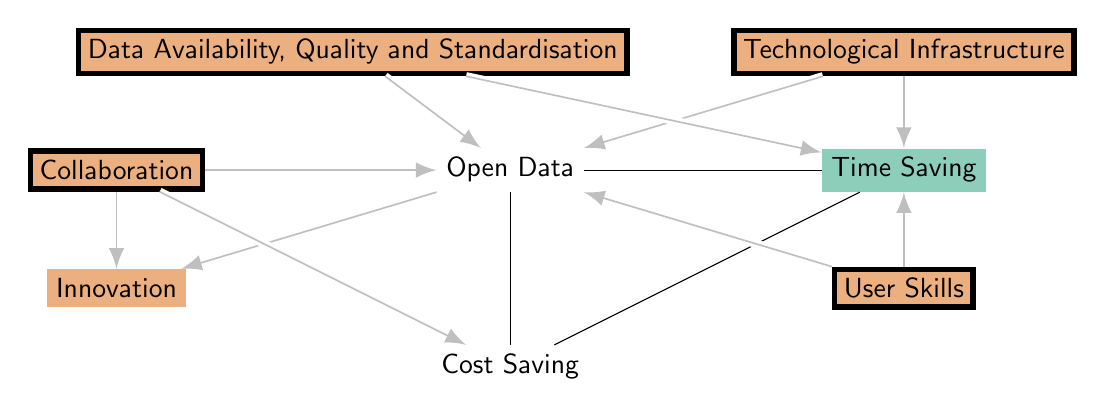
\begin{tikzpicture}

% Nodes
\node                     (open data)      at (-3, -1.5) {Open Data};
\node                     (cost saving)    at (-3,-4)    {Cost Saving};
\node[open]               (time saving)    at (2, -1.5)  {Time Saving};
\node[closed,conditioned] (user skills)    at (2,-3)     {User Skills};
\node[closed]             (innovation)     at (-8, -3)   {Innovation};
\node[closed,conditioned] (collaboration)  at (-8, -1.5) {Collaboration};
\node[closed,conditioned] (infrastructure) at (2, 0)     {Technological Infrastructure};
\node[closed,conditioned] (quality)        at (-5, 0)    {Data Availability, Quality and Standardisation};

% Edges
\draw (quality)        edge[e-gray] (open data)
      (infrastructure) edge[e-gray] (open data)
      (collaboration)  edge[e-gray] (open data)
      (open data)      edge         (cost saving)
      (open data)      edge         (time saving)
      (collaboration)  edge[e-gray] (innovation)
      (open data)      edge[e-gray] (innovation)
      (collaboration)  edge[e-gray] (cost saving)
      (time saving)    edge         (cost saving)
      (user skills)    edge[e-gray] (open data)
      (user skills)    edge[e-gray] (time saving)
      (infrastructure) edge[e-gray] (time saving)
      (quality)        edge[e-gray] (time saving);

\end{tikzpicture}

\end{document}
